\documentclass[12pt]{article}
\usepackage[utf8]{inputenc}
%%%%%%%%%%%%%%%%%%%%%%%%%%%%%%%%%%%%%%%%%
% Homework Template
% Author: Nayeong Kim
%%%%%%%%%%%%%%%%%%%%%%%%%%%%%%%%%%%%%%%%%

%----------------------------------------------------------------------------------------
%	PACKAGES
%----------------------------------------------------------------------------------------
\usepackage{geometry}
\usepackage{amsmath}
\usepackage{graphicx}
\usepackage{amssymb}
\usepackage{amsthm,cite}
\usepackage{multirow}
\usepackage{float}
\usepackage{tikz}
\usepackage{caption}
\usepackage{subcaption}
\usepackage{xfrac}
\usepackage{tikz-cd}
\usepackage{setspace}


%----------------------------------------------------------------------------------------
%	MATH ENVIRONMENTS
%----------------------------------------------------------------------------------------
\theoremstyle{definition}
\newtheorem{theorem}{Theorem}
\newtheorem{corollary}{Corollary}
\newtheorem{definition}{Definition}
\newtheorem{example}{Example}
\newtheorem{proposition}{Proposition}
\newtheorem{claim}{Claim}
\newtheorem{exercise}{Exercise}
\newtheorem{lemma}{Lemma}
\newtheorem{question}{Question}
\newenvironment{solution}{\begin{proof}[Solution]}{\end{proof}\noindent \\}

%--------------------------------------------------------------------------------------
%	MATH SYMBOLS
%----------------------------------------------------------------------------------------
\newcommand{\Z}{\mathbb{Z}}
\newcommand{\N}{\mathbb{N}}
\newcommand{\Q}{\mathbb{Q}}
\newcommand{\R}{\mathbb{R}}
\newcommand{\C}{\mathbb{C}}
\newcommand{\A}{\mathbb{A}}
\newcommand{\F}{\mathbb{F}}
\newcommand{\Act}{\rotatebox[origin=c]{180}{$\circlearrowright$}}
\newcommand{\nil}{\mathrm{nil}}
\newcommand{\rad}{\mathrm{rad}}
\newcommand{\ann}{\mathrm{ann}}
\newcommand{\im}{\mathrm{im}}
\newcommand{\Hom}{\mathrm{Hom}}
\newcommand{\Cont}{\mathrm{cont}}
\newcommand{\Ass}{\mathrm{Ass} \ }
\newcommand{\Tr}{\mathrm{trace}}
\newcommand{\gr}{\mathrm{gr}}
\newcommand{\inform}{\mathrm{in}} % initial form
\newcommand{\codim}{\mathrm{codim}}

%--------------------------------------------------------------------------------------
%	TITLE
%----------------------------------------------------------------------------------------
\newcommand{\maketitletwo}[2][Spring 2022]{\begin{center}
            \large{\textbf{#1}}\\
            \Large{\textbf{#2}} % Name of course here
            \vspace{10pt}
            
            \normalsize{\hfill Nayeong Kim  % Your name here
    	}        % Change to due date if preferred
    	\vspace{15pt}
    \end{center}}
\onehalfspacing
\begin{document}
\maketitletwo[Spring 2023]{Combinatorics: Homework 3}
\vspace{-30pt}
\subsection*{PART I}
\subsubsection*{Problem 1}
How many subsets of $\{1,2,3,4,5,6,7,8,9\}$ have an odd number of elements?
\begin{solution}
We realize that every subset $A$ with an even number of elements has the complement $A^c$ with an odd number of elements. Every subset appears in exactly one of such pairs hence the number of such subset is the half of the number of all subsets of $\{1,2,3,4,5,6,7,8,9\}$. Therefore $2^9/2 = 256$.
\end{solution}

\vspace{-50pt}
\subsubsection*{Problem 2}
A country is designing a flag with three horizontal stripes of equal heights. Each stripe should be red, white, blue, or yellow, and no two adjacent stripes should have the same color. How many possible flags are there?
\begin{solution}
We observe that there are 4 choices for the center stripe. And the top and bottom ones have 3 choices and the choice of the top color is independent from the bottom one. Therefore there are $4 \times 3 \times 3 = 36$ possible flags.
\end{solution}

\vspace{-50pt}
\subsubsection*{Problem 3}
How many ways are there to list the letters of the word ALABAMA?
\begin{solution}
The number of letters is $7$ and the only repeated letters are $4$ of A. So the number of ways is 
\begin{align*}
    \frac{7!}{4!} = 210.
\end{align*}
\end{solution}

\subsubsection*{Problem 4}
In countries that currently belong to the European Union, 17 languages are spoken by at least ten million people. For any two of these languages, the European Commission employs an interpreter who can translate documents from one language to the other, and vice versa. One journalist has recently noted that when the soon-to-be admitted countries bring the number of languages spoken by at least ten million people in the Union to 22, more than a hundred new interpreters will be needed. Was she right? (No interpreter works two jobs.)
\begin{solution}
No. If there are $n$ languages, we can see that the number of interpreters must be ${n \choose 2}$. So we need ${22 \choose 2} - {17 \choose 2} = 231 - 136 = 95$ new interpreters.
\end{solution}
\vspace{-50pt}

\subsubsection*{Problem 5}
A student in physics needs to spend five days in a laboratory during her last semester of studies. After each day in the lab, she needs to spend at least six days in her office to analyze the data before she can return to the lab. After the last day in the lab, she needs ten days to complete her report that is due at the end of the last day of the semester. In how many ways can she do this if we assume that the semester is 105 days long?
\begin{solution}
We assume that she has to spend each day in the lab or in the office. She needs $1 + 6 + 1 + 6 + 1 + 6 + 1 + 6 + 1 + 10 = 39$ days for doing lab and data analysis. Then we can divide $105 - 39 = 66$ days into $6$ intervals which is divided by the $5$ lab days (allowing $0$ interval). The number of ways is the same as the number of choosing $5$ from $67$ allowing repetition. So the number is
\begin{align*}
    {67+5-1 \choose 5} = \frac{71 \cdot 70 \cdot 69 \cdot 68 \cdot 67}{5!} = 13019909.
\end{align*}
\end{solution}
\subsection*{PART II}
\subsubsection*{Problem 1}
Let $n=p_1^{a_1} p_2^{a_2} \cdots p_k^{a_k}$, where the $p_i$ are distinct primes, and the $a_i$ are $k$ positive integers. How many positive divisors does $n$ have?
\begin{solution}
We can write any positive divisor as $m=p_1^{b_1} p_2^{b_2} \cdots p_k^{b_k}$ where we have $0 \leq b_i \leq a_i$. The choice of $b_i$ is independent from the choice of $b_j$ where $i \neq j$ and the number of possible choices of $b_i$ is $a_i+1$. Therefore the number of positive divisors of $n$ is $\prod_{i=1}^k (a_i+1)$.
\end{solution}
\vspace{-20pt}
\subsubsection*{Problem 2}
We want to select three subsets $A, B$, and $C$ of $[n]$ so that $A \subseteq C, B \subseteq C$, and $A\cap B \neq \emptyset$. In how many different ways can we do this?
\begin{solution}
We will count the number by subtracting the number of $A, B \subseteq C \subseteq [n]$ without any condition from the number of such cases with $A\cap B = \emptyset$.

\begin{table}[h!]
    \centering
    
\begin{tabular}{cc}
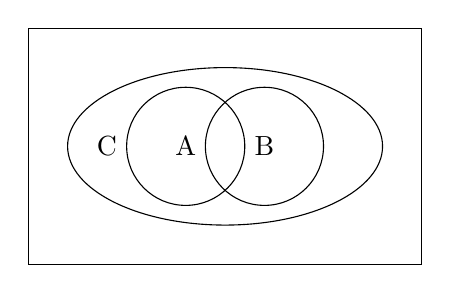
\begin{tikzpicture}
\node[rectangle, draw=black, minimum width = 5cm, 
    minimum height = 3cm] (r) at (0,0) {};
\node[draw, circle, minimum size = 1.5cm] (A) at (-0.5,0) {A};
\node[draw, circle, minimum size = 1.5cm] (B) at (0.5,0) {B};
\draw (0,0) ellipse (2cm and 1cm);
\node (C) at (-1.5, 0) {C};
\end{tikzpicture}
&
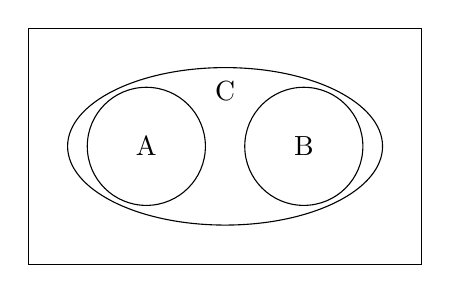
\begin{tikzpicture}
\node[rectangle, draw=black, minimum width = 5cm, 
    minimum height = 3cm] (r) at (0,0) {};
\node[draw, circle, minimum size = 1.5cm] (A) at (-1,0) {A};
\node[draw, circle, minimum size = 1.5cm] (B) at (1,0) {B};
\draw (0,0) ellipse (2cm and 1cm);
\node (C) at (0, 0.7) {C};
\end{tikzpicture}\\
Figure 1 & Figure 2
\end{tabular}
\end{table}


We realize that the first one is allocating $n$ elements into the $5$ regions in Figure 1 and the second one is allocating $n$ elements into the $4$ regions in Figure 2. Therefore the number is $5^n - 4^n$.
\end{solution}

\subsubsection*{Problem 3}
Let $P$ be a convex $n$-gon in which no three diagonals intersect in one point. How many intersection points do the diagonals of $P$ have?
\begin{solution}
We observe that there is a bijection between the set of intersection points and the set of choosing $4$ from $n$ vertices. When we pick an intersection point of two diagonals, we can pick the $4$ vertices from the two diagonals. When we pick any $4$ vertices, we can consider a convex $4$-gon having the $4$ vertices and its two diagonals, which are also diagonals of the given $n$-gon, has one intersection. Therefore the number is $n \choose 4$.
\end{solution}

\subsubsection*{Problem 4}
A store has n different products for sale. Each of them has a different price that is at least one dollar, at most $n$ dollars, and is a whole dollar. A customer only has the time to inspect $k$ different products. After doing so, she buys the product that has the lowest
price among the $k$ products she inspected. Prove that on average, she will pay $(n+1)/(k+1)$ dollars.
\begin{solution}
We can consider choosing $k+1$ from $0, \cdots, n$ and remove the smallest element. Then the outcome is $k$ chosen numbers from $1, \cdots, n$ with the weight $r$ when $r$ is the smallest number among last numbers. We realize that this is the same as the total price of the whole cases. Hence the average value is ${n+1 \choose k+1} / {n \choose k} = (n+1)/(k+1)$.
\end{solution}

\subsubsection*{Problem 5}
How many $n \times n$ square matrices are there whose entries are $0$ or $1$ and in which each row and column has an even sum?
\begin{solution}
If we fill the most left top submatrix of size $n-1 \times n-1$, the last numbers of $n-1$ rows and $n-1$ columns are decided. We can see that the parity of the sum of the last elements of $n-1$ rows is the same as the parity of the sum of the last elements of $n-1$ columns. It implies that the parity of $n, n$-th element is decided. In other words, it is free to choose $0$ or $1$ of the most left top $n-1 \times n-1$ entries and the other entries are decided when the $n-1 \times n-1$ submatrix is decided. Therefore the number is $2^{(n-1)^2}$.
\end{solution}
\end{document}
